\subsection{問題設定}
本実験でFPGA上で実装するテーマとして、巡回セールスマン問題を選択した。
いくつかあるバリエーションのうち、本実験では、以下のように問題設定を行った。
\begin{itembox}[l]{問題設定}
    256×256のマス目上に、ランダムに配置された64個の点がある。
    これらの点をすべてめぐって元の点に戻ってくるような閉路(ハミルトン閉路)のうち、
    総距離ができるだけ小さいものを求めよ。
\end{itembox}
例えば、図\ref{fig:tspsapmle}においては、右図は左図に比べ総距離が小さく評価が高い。
\begin{figure}[h]
    \begin{center}
        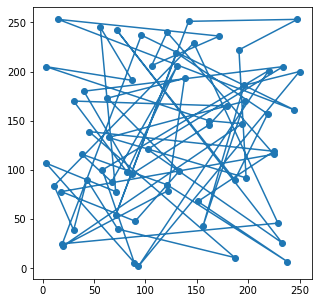
\includegraphics[width=7cm]{figure/tsp_bad.png}
        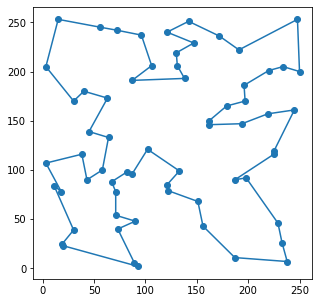
\includegraphics[width=7cm]{figure/tsp_good.png}
        \caption{
            今回の問題設定における巡回セールスマン問題の例\\
            (左) 総距離が大きい経路(総距離: 8437.0)
            (右) 総距離が小さい経路(総距離: 1748.6)
        }\label{fig:tspsapmle}
    \end{center}
\end{figure}

\subsection{巡回セールスマン問題の解法}
巡回セールスマン問題は、NP困難であることが知られている。つまり、厳密な最適解を多項式時間で求めることはできない。
頂点数が20程度の小さな問題であれば動的計画法によって最適解を求めることができるが、それ以上の規模ではヒューリスティックな手法を用いて最適解に近づける手法が主となる。
ヒューリスティックな手法の多くは、局所探索法の考え方に基づいている。
\subsubsection{局所探索法}\label{sec:local}
局所探索法とは、ある解から出発して、その近傍解(一部を変えた解)を探索することを繰り返すことで、最適解に近づける手法である。\cite{HouTengYouTaiXunHuiserusumanWenTiTSPNoJiBenDenaJiekiFang2021}
近傍解の生成方法には様々な種類があり、それぞれ最適解へのたどり着きやすさ・生成に要する時間・並列可能性などの特徴が異なる。
そのうち最もシンプルな方法が、経路のうち2つの頂点を入れ替えることで近傍解を生成する方法である。
例えば、図\ref{fig:tspswap}において、元々の経路(左図)の一部に1→5→3という部分と4→2→6という部分があったとき、右図のように1→2→3と4→5→6という経路に変更することで近傍解を生成する。
この変更は、経路の2と5を入れ替えることで実現でき、生成にかかるコストが非常に低い。また、この方法は並列可能性がとても高い。
二点を入れかえるべきかどうかを計算するには、入れかえる2点と、それぞれの前後の点の計6点の情報がわかっていれば良い。
これら6点が重複しないように選択すれば、複数の箇所について同時に近傍を生成し、判定・更新を行うことができる。
例えば図~\ref{fig:tspswapparallel}において、青で示した部分と赤で示した部分は独立に判定・更新可能である。
\begin{figure}[h]
    \begin{center}
        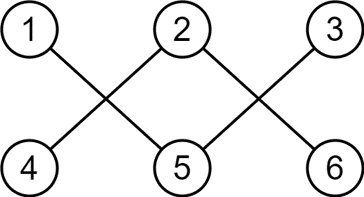
\includegraphics[width=6cm]{figure/swap_bad.png}
        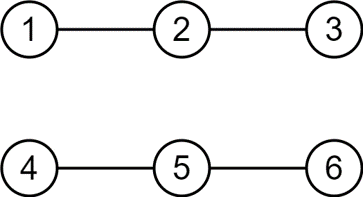
\includegraphics[width=6cm]{figure/swap_good.png}
        \caption{
            (左)交換前の経路[1→5→3 / 4→2→6]
            (右)交換後の経路[1→2→3 / 4→5→6]
        }\label{fig:tspswap}
    \end{center}
\end{figure}

\begin{figure}[h]
    \begin{center}
        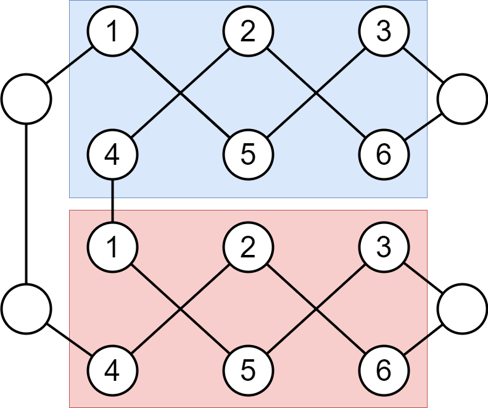
\includegraphics[width=6cm]{figure/parallel_swap_bef.png}
        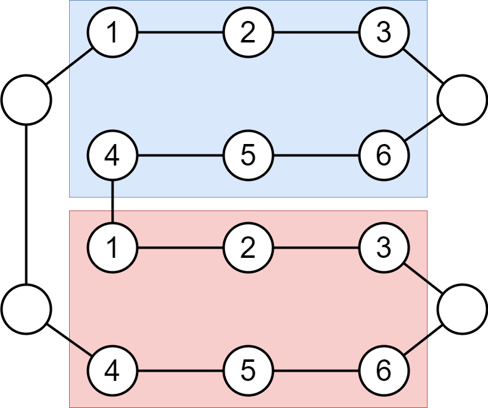
\includegraphics[width=6cm]{figure/parallel_swap_aft.png}
        \caption{
            複数の箇所について同時に近傍を生成し、判定・更新を行う例
        }\label{fig:tspswapparallel}
    \end{center}
\end{figure}

ランダムな近傍を繰り返し生成し、総距離が小さくなるような近傍を見つけたら、貪欲にその近傍に移動することを繰り返すことで、最適解に近づける方法を山登り法と呼ぶ。

\subsubsection{山登り法のデメリットとその対策}
山登り法は、局所最適解に陥りやすいという欠点がある。
局所最適解とは、ある解の近傍にあるいずれの解によっても結果が改善しない解のことである。これは必ずしも最適解とは限らない。

結果が改善する近傍のみを採用する山登り法では、局所最適解に陥ると、そこから脱出することができなくなる。この問題に対しては以下のような手法が存在する。\cite{HouTengYouTaiXunHuiserusumanWenTiTSPNoJiBenDenaJiekiFang2021}
\begin{itemize}
    \item 焼き鈍し法: 結果が改善する近傍を必ず採用することに加え、結果が改善しない近傍も一定の確率で採用することで、局所最適解に陥りにくくする手法
    \item 反復局所探索法: 山登り法によって局所最適解に陥ったら解の一部分を崩す、という操作を繰り返すことで、局所最適解に陥りにくくする手法
\end{itemize}
これらの手法を用いれば、山登り法の欠点をある程度解消し、かなり精度の高い解を得ることができる。

\subsection{実験目標}\label{sec:goal}
ここまでに示した内容を踏まえ、今回の実験では以下の目標を設定した。
\begin{itembox}[h]{目標}
    \begin{enumerate}
        \item FPGA上で巡回セールスマン問題に対する山登り法を実装し、局所最適解を得る。
        \item 1. の実装を並列化し、CPU上で動作するプログラムと比較して高速化を図る。
        \item 2. の実装を改良し、焼き鈍し法または反復局所探索法を実装することで、局所最適解に陥ることなく最適解に近づける。
        \item VGA出力を用いて、経路の変化をリアルタイムに表示する。
    \end{enumerate}
\end{itembox}
ハードウェア実装の強みは並列可能性の高さであり、それを活かした高速化を行うことが本実験の趣旨であることから、特に2.の実装に注力した。
成果については、局所最適解に陥るまでに要する時間を比較し、高速化の程度を示すこととする。
